% Basic LaTeX template for NE 204 lab report
\documentclass[11pt]{article}

%==============================================================================
%%% Everything between the "="'s is the preamble.
%%% Define packages and meta data here

% Common packages
\usepackage{amsmath}    % Expanded math
\usepackage{amssymb}    % Expanded math symbols
\usepackage{graphicx}   % For images
\usepackage[margin=1.25in]{geometry}
%\usepackage[version=3]{mhchem} % For nuclide formatting

% All images/figures will be stored in the images folder.
% Specify that here so pdflatex knows where to look for images.
\graphicspath{{./images/}}

% Metadata
\title{Lab 0}
\author{Joanna Szornel}
\date{\today}
%==============================================================================

\begin{document}

% Compile metadata from preamble into a nicely-rendered title section
\maketitle

% The *'s next so section/subsection definitions suppresses numbering
\section*{Introduction}
\label{sec:intro}
In this work, a digital trapezoidal filter was implemented for gamma-ray spectroscopy with a coaxial HPGe detector. A digital rather than analog implementation allows for greater ease and flexibility in tuning parameters. The two parameters of the filter that can be optimized are the peaking time and the gap time. Often in applications a trade-off between rate performance and energy resolution must be made.  Here the filter is being tuned to achieve the best possible energy resolution, disregarding rate performance. Then, using the optimized filter on spectral data from several calibration sources, the Fano factor was calculated.

In common HPGe detector configurations, a charge-sensitive preamplifier integrates the charge induced on an electrode and outputs a voltage proportional to the collected charge. A feedback resistor and capacitor provide an RC circuit which causes an exponential decay of the preamplifier's output signal. These pulses are shaped before further processing to eliminate their long decay tail while preserving information about signal amplitude, timing and signal shape.

Although theoretically cusp or triangular filters give better noise performance, trapezoidal filters are more commonly used. This is due partially to the impracticality of digitizing a signal with a small flat top. Additionally, the trapezoidal filter is advantageous for detectors which see variable charge collection time as the flat top can be tuned to avoid ballistic deficit \cite{Knoll}.

Due to the random nature of radioactive decay, even at low count rates pile-up must be considered. To prevent pile-up, shaped pulses should be kept short, minimizing peaking and gap times. However, making these parameters too short can lead to incomplete charge collection or poor noise performance. Making these parameters too long can lead to pile-up or poor noise performance.

This is because of the dependance on peaking time of the three main contributions to the electronic noise- series noise, parallel noise and 1/$f$ noise. The series noise $\propto \frac{1}{\tau}$. The parallel noise is $\propto\tau$. The 1/$f$ noise is independent of $\tau$. Thus a balance between the noise contributions must be found for some optimal $\tau$. 



\section*{Methods}
\label{sec:meth}
\subsection*{Data Collection}

A Struck Integrated Systems (SIS) 3302 DAQ module was used to collect data. This module has 16-bit ADCs and an internal 100 MHz clock which was used for all of the measurements. Preamplifier output signals were fed directly to the DAQ module without additional processing. These output signals were digitized and used to perform this analysis. Additionally, the on-board shaping amplifier was used to retrieve event energies (in ADC units).

The trigger threshold value was set so that gamma-ray pulses with energies as low as approximately 50 keV could be collected without excessive noise and without exceeding the voltage range of the DAQ. Data was collected attempting to have negligible pile-up effects. The event rate was chosen to be approximately 800 Hz (triggers) for a system with a 100 MHz clock (10 ns sampling time) and a preamplifier pulse decay time of roughly 50 $\mu$s.

Before further processing each pulse was baseline corrected. This was done by subtracting the average value of the first 15 samples from all of the samples in that pulse.

\subsection*{Energy Calibration}

Before taking spectral data, each channel must be calibrated. The 661.7 keV line from ${}^{137}$Cs and the 59.5 keV line from ${}^{241}$Am were used to perform a linear energy calibration.

Four calibration data sets were taken. First an ${}^{241}$Am source was placed near the outward face of detector 1. Next, the source was moved to the outward source of the detector 2. This was repeated with a ${}^{137}$Cs source. This was done to ensure that all channels would have spectral data for both sources.

Two spectra were plotted for each channel, one using both ${}^{241}$Am data sets combined, and the other using both ${}^{137}$Cs data sets combined. A region of interest around each photopeak was selected by visual inspection of the relevant spectrum. These regions were each fit with a Gaussian function and a linear function (to account for background) using the built in models in LmFit \cite{LMFIT}. A linear energy calibration was used.

Channels which had fewer than 50 total counts around the ${}^{137}$Cs peak or showed other strange behavior (visually observed) in spectra were not calibrated, and were not used in any of the analysis shown. This included 22 of the 152 channels. Most of these channels correspond to strips near the edge of the detectors which have been disconnected due to high leakage currents. The two channels with the highest FWHM values had very few events in the cesium photopeak region, leading to poor fitting. Channels with a 0 FWHM are those which were not calibrated.

The energy resolution of each channel is determined from the FWHM of the peak. This is shown in figure \ref{fwhm}. Each individual channel had a low number of counts in the photopeak ($\approx$ 60). The error bars shown correspond to fitting errors. Low statistics in the cesium peaks limited this procedure (there were roughly 60 counts for a single channel). The average energy resolution was found to be 2.44 keV., with a standard deviation of 0.51 keV. The channels with high FWHM values tend to be those with a small number of counts in the peak. The variation between channels would likely decrease with better statistics.  Using a larger cesium dataset results in a better energy calibration. This was done in \ref{fwhm_long}. The average energy resolution was found to be 2.37 keV., with a standard deviation of 0.39 keV. Ideally, all strips would have the same energy resolution. Realistically, however, we expect that some strips, in particular those on the outer edges of the detector, to have degraded energy resolution. The DC face of detector 1 contains channels 0 through 37. Here we see a u-shaped trend in the energy resolution, potentially demonstrating the effects of higher leakage current near the edges.

\begin{figure}[h]
\begin{centering}
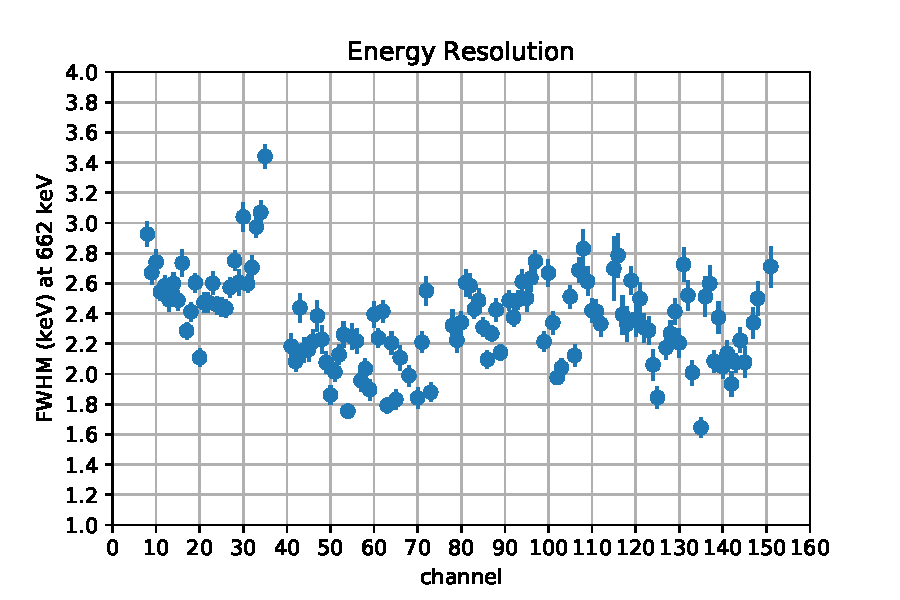
\includegraphics[width=0.7\textwidth]{./figures/energy_res.pdf}
\caption{The energy resolution for each channel of two double-sided strip detectors. Channels with a 0 FWHM are those which were not calibrated due to low statistics, high leakage currents, or other issues. The error bars shown correspond to fitting errors.}
\label{fwhm}
\end{centering}
\end{figure}

\begin{figure}[h]
\begin{centering}
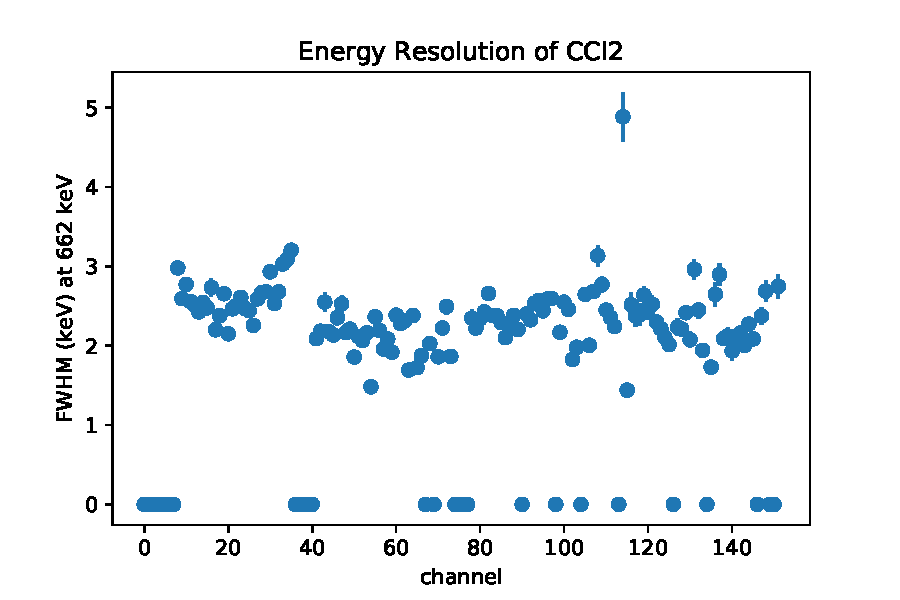
\includegraphics[width=0.7\textwidth]{./figures/energy_res_long.pdf}
\caption{The energy resolution for each channel of two double-sided strip detectors. Channels with a 0 FWHM are those which were not calibrated due to low statistics, high leakage currents, or other issues. The error bars shown correspond to fitting errors.}
\label{fwhm_long}
\end{centering}
\end{figure}

\subsection*{Timing}

A distribution of trigger times over all events and both detectors was plotted. For a Poisson process, the distribution of arrival times is exponential, peaked at zero and falling more steeply with increasing rate (the decay constant of the exponential function is $\lambda = 1/mean rate)$. 

The distribution for experimental triggers does not follow this trend exactly. There are more events near 0 and more events at 1 than at zero. This has to do with the fact that for each event which causes a trigger on a strip, it is very likely to see triggers on other strips (from image charges on neighboring strips, signals from the electrodes on the opposite face or in the other detector, noise, charge-sharing, etc.). It is found that most events occur within 250 nanoseconds of each other. The expected drift time for charges within a detector of this type and size is on the order of hundreds of nanoseconds. This agrees with what is observed. 

\begin{figure}[h]
\begin{centering}
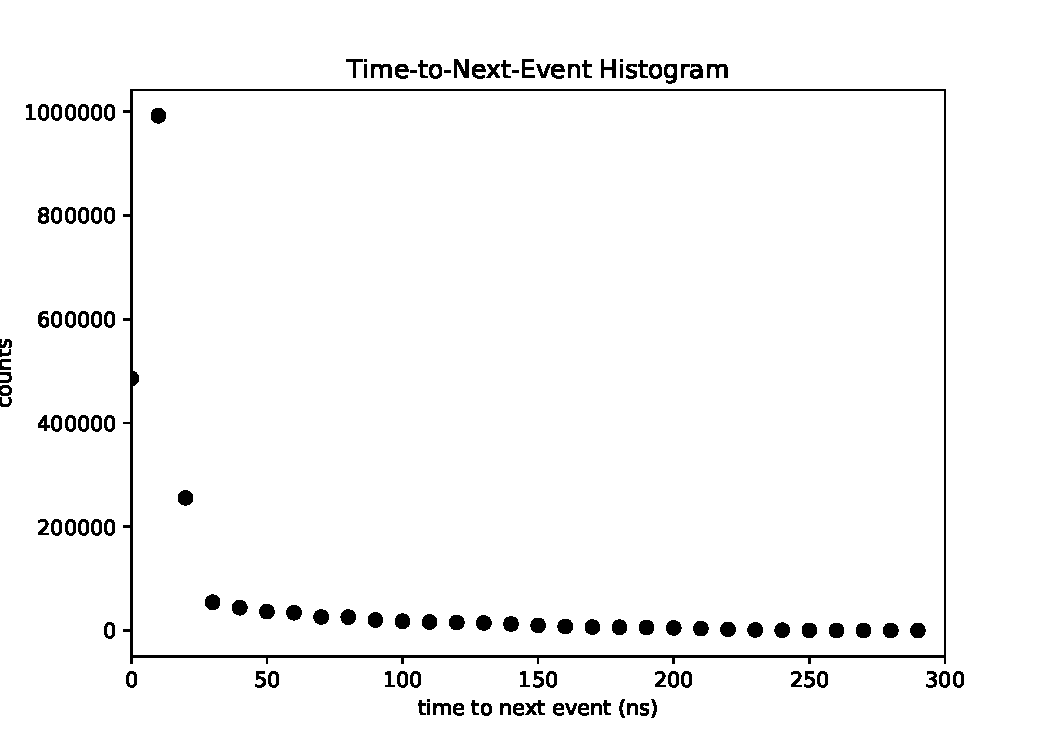
\includegraphics[width=0.7\textwidth]{./figures/time-to-next-event.pdf}
\caption{The energy resolution for each channel. Channels with a 0 FWHM are those which were not calibrated. The error bars shown correspond to fitting errors.}
\label{timehist}
\end{centering}
\end{figure}

To select single-site events, events which have triggers within 400 ns of each other on opposite faces of a detector crystal were selected. This is a generous window, as we expect the drift time for charge carriers within this detector to be $\approx$100-200ns \ref{knoll}. Requiring this, along with full energy deposition, provided the selection criteria for a single-site event.

For an event, each of the two pulses (from the opposite faces) was smoothed using a Savitzky-Golay filter \cite{scipy}. The last point where the smoothed signal did not exceed 50 percent of its maximum value and 6 neighboring points (3 to each side) were fit with a linear function. The time that this linear function crossed 50 percent was calculated and used as $t50$. The $t50$ value of one face was subtracted from the other, to find $\Delta t50$. Here the $t50$ of the electrons was subtracted from that of the holes ($t50_{cathode}- t50_{anode}$). The difference in trigger time was added to $\Delta t50$ to find the difference in signal arrival times.

\begin{figure}[h]
\begin{centering}
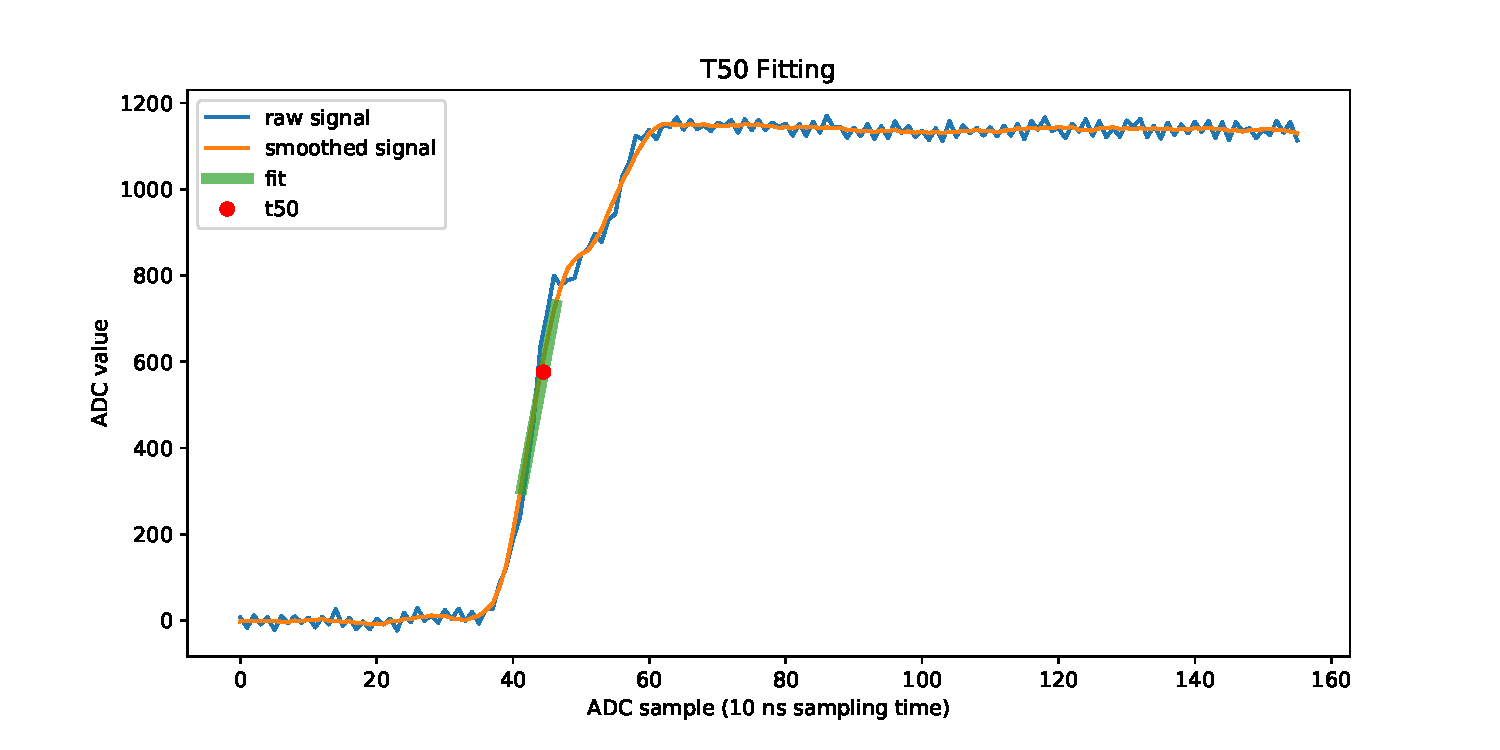
\includegraphics[width=0.7\textwidth]{./figures/t50_fitting.pdf}
\caption{Each raw signal (blue) is smoothed with a Savitzky-Golay filter (orange). The region around the point at which the smoothed signal exceeds half its maximum is fit with a line (green) to extract the t50 value (red point)}
\label{fit}
\end{centering}
\end{figure}

\subsection*{Depth Determination}

${}^{137}$Cs was used to ensure events throughout the potential range of detector depth. Additionally, these signals have greater SNR which makes it easier to properly trigger on and correlate signals.

The maximum $\Delta t50$was seen to be roughly 210, the minimum $\Delta t50$ was seen to be -160. For a rough determination of the depth, the maximum value is assumed to correspond to the anode and the minimum value to the cathode. A linear fit is applied to determine intermediate position values. This is not a fully representative treatment. It fails to take into account effects due to the non-linear weighting potential directly near electrodes, different charge carrier mobilities, realistic charge transport, and other effects. However, for the purposes of this work, we make this crude assumption following \cite{amman}.

A different linear interpretation was used as well. Following \cite{cci21}, assuming saturation velocity for both charge carriers, one can use a linear function to relate depth ($z$) to $\Delta t50$:

\begin{equation}
$z = z_0 + k \Delta t50$
\end{equation}

where z is the depth of the interaction, $z_0$ is a constant depth which is slightly offset from the midpoint of the detector to account for differences in electron and hole velocities, and $k$ is a proportionality factor. $z_0$ and $k$ were experimentally determined for detector 1 to be 5.2 mm and 0.04 mm/ns respectively, in \cite{cci21}. This offset of 5.2 mm was adjusted to 5.95 mm to better fit the data set.


\section*{Results}
\label{sec:res}
\subsection{Timing}

\begin{figure}[h]
\begin{centering}
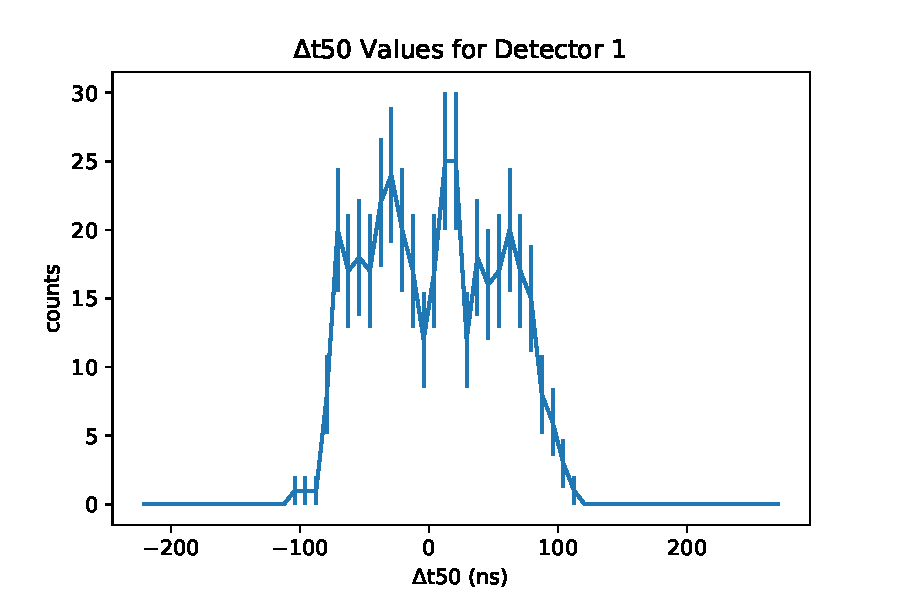
\includegraphics[width=0.7\textwidth]{./figures/t50s_det1.pdf}
\caption{The $\Delta t50$ distribution for detector 1.}
\label{t50_1}
\end{centering}
\end{figure}

ADD CAPTION STUFF TO THESE 2 The source was located on the DC side of detector1. We expect to see an exponential fall-off of events as depth increases from this point. The

\begin{figure}[h]
\begin{centering}
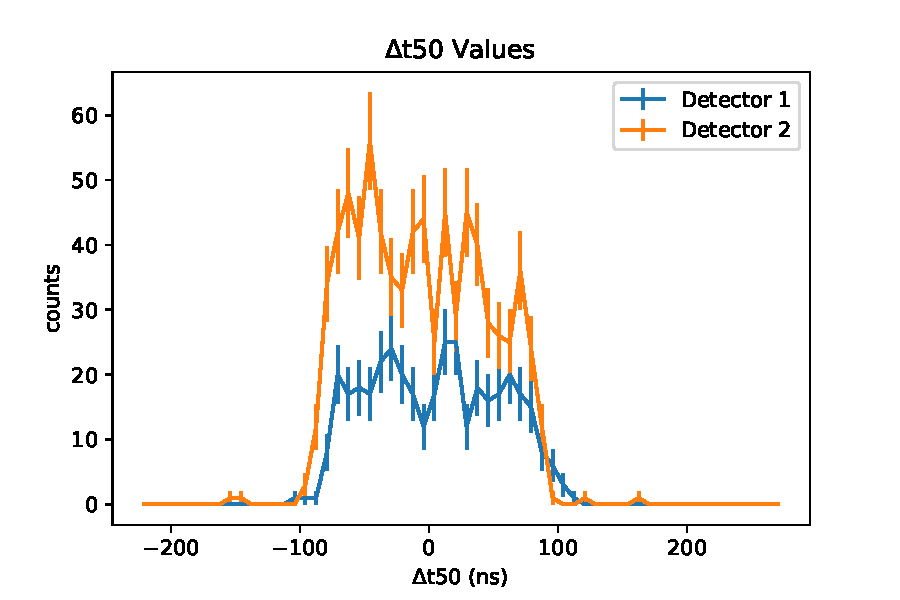
\includegraphics[width=0.7\textwidth]{./figures/t50s_det2.pdf}
\caption{The $\Delta t50$ distribution for detector 2.}
\label{t50_2}
\end{centering}
\end{figure}

The trigger time of a signal is determined by a on-board fast trapezoidal shaper. This trigger time may differ slightly between signals, depending on the location of the interaction, leading to additional uncertainty. The effect of this jitter will be studied for more precise position determination.

\subsection{Depth Determination}

-depth profile with theoretical curve for comparison

\begin{figure}[h]
\begin{centering}
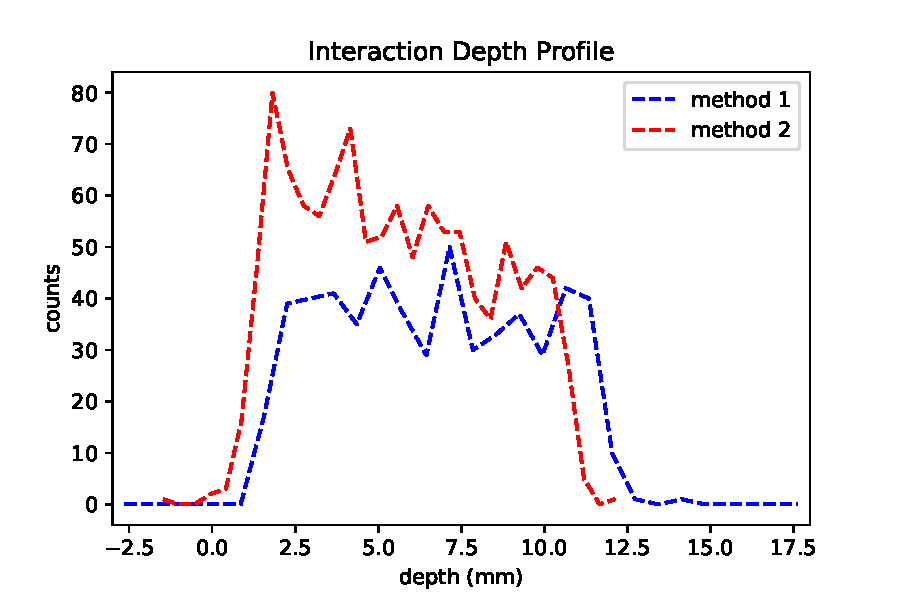
\includegraphics[width=0.7\textwidth]{./figures/interactiondepths.pdf}
\caption{The $\Delta t50$ distribution for detector 2.}
\label{t50_2}
\end{centering}
\end{figure}

The depth profile for detector 1 is shown in \ref{interactiondepths}. The second method of calculating depth, which takes into account the different carrier velocities, seems to give a better result. More events are confined within the detector and the depth profile looks to have a stronger exponential trend.

Some events will be subject to charge sharing, charge loss in the inter-strip gap, collection to a disconnected strip, etc. If the total charge gathered on one side of the detector by the main collecting electrode is not great enough, the signal may not be recorded. This leads to 

Another source of error is scattering events. A gamma ray may scatter in an event with full-energy deposition (forward Compton scattering within a voxel for example), and the assumption of a single scattering event where there were two or more will lead to an improperly reconstructed interaction position. This is another source of error in our measurement. However, with the Geant4 data, we have determined that 

\subsection{Comparison to Simulation}

A simple model was built in GEANT4 (two planar HPGe crystals, 74 mm wide, 15 mm thick, 10 mm apart). No surrounding material was included in the model. A point source emitting gamma-rays with energy 661.657 keV from a point 2 meters in front of the front-face of the first detector was used \cite{ebss}. This data was used to compare to the experimentally determined distribution of interaction depths.

\section*{Discussion}
\label{sec:disc}
\subsection*{Summary}

Timing information was extracted and 

which method was best

\subsection*{Future Work}

There are many potential improvements and future steps that could be taken. The spread in signal trigger time will be investigated, as it may have an effect of the $\Delta t50$ values calculated. Additionally, many channels which were ignored in this work could be calibrated with more data and more careful fitting of each individual channel.

More sophisticated pulse shape analysis methods could be applied to achieve better position determination. Utilizing a more complex function (such as the inverse sigmoid function shown in \cite{cci21}, would likely give better results. A typical pulse shape analysis technique in experiments like GRETINA is to model fields in the detector, generate a library of expected signals, and by comparing to these signals and interpolating, determine interaction positions. This technique will be compared to the simple linear method used here, to evaluate its advantages. A model of the detector and a signal library (for depth information only) has been built with  ADL3 \cite{adl3}. Using the GEANT4 data discussed earlier, interactions could be simulated at realistic positions. The resultant signals could be treated as experimental data to compare against the reference signals and check how useful this library approach is at determining interaction positions.

Here we have focused only on the depth of interaction. The lateral position can be determined through simple methods like taking the ratio of image charges on neighboring strips to the collecting electrode, or through more complex methods like the signal library method described above. Here, the lateral position determination proved difficult due to the worse SNR of image charge signals, the high number of uncalibrated channels, and suspected cross-talk. However, through more careful event selection, lateral position determination methods could be studied.

Lastly, using collimation to acquire events are specific locations would provide a verification and comparison of these methods.


% Bibliography
\bibliographystyle{plain}
% Refers to a bibtex file in the current dir named "references.bib"
\bibliography{references}

\end{document}
